\subsection{Comparison on Try-Catch Necessity Checking Effectiveness (RQ1)}
%\label{sec:rq1}

\begin{table}[t]%[htpb]
  \caption{Try-Catch Block Comparison with XRank (RQ1)}
  \vspace{-12pt}
  \small
	\begin{center}
		\renewcommand{\arraystretch}{1}
		\begin{tabular}{| p{3.05cm}<{\centering} | p{1.2cm}<{\centering} | p{1.2cm}<{\centering}| p{1.2cm}<{\centering}|}
		  \hline
			Github dataset  & Precision  &  Recall & F1-score \\
			\hline
%			CodeBERT w/o fine-tuning & 0.4969  & \textbf{0.9719}   & 0.6576\\
			\hline
			XRank & 0.810 & 0.530 & 0.630\\
			\hline
			\tool   &  \textbf{0.981} &  {\bf 0.984} & \textbf{0.982}\\
			\hline
		\end{tabular}
		\label{tab:xblock-1}
	\end{center}
\end{table}

\begin{table}[t]%[htpb]
  \caption{Try-Catch Block Comparison with GPT-3.5 (RQ1)}
  \vspace{-12pt}
  \small
	\begin{center}
		\renewcommand{\arraystretch}{1}
		\begin{tabular}{| p{1.85cm}<{\centering} | p{1.6cm}<{\centering} | p{1.6cm}<{\centering}| p{1.6cm}<{\centering}|}
		  \hline
		Small dataset	  & Precision  &  Recall & F1-score \\
			\hline
			GPT-3.5  & 0.666--0.804  & 0.726--0.778   & 0.695--0.791\\
			\hline
			\tool   &  \textbf{0.994} &  {\bf 1.0} & \textbf{0.997}\\
			\hline
		\end{tabular}
		\label{tab:xblock-2}
	\end{center}
\end{table}


%{\color{red}{This section waiting for the XRank Results. But from the current estimate, our approach should have higher F-score. But the recall and precision I'm not sure. Once I have the results, I will update this section.}}

%Table~\ref{tab:xblock} displays the comparison result.

As seen in Table~\ref{tab:xblock-1}, {\tool} achieves very high
Precision, Recall and F-score on the Github dataset---all above
98\%.
%In comparison, the CodeBERT baseline model has a much lower
%Precision, around 50\%. However, it achieves a slightly higher
%Recall. After examining the result, we find that the model
%overwhelmingly predicts that the input
%code snippet contains a \code{try-catch} block: In our balanced test
%dataset that contains 30,764 samples, only 236 samples receives the
%negative label (i.e., no \code{try-catch}) from CodeBert.
In comparison, {\tool} relatively improves over XRank {\bf 21\%, 85.7\%,
and 55.9\%} in Precision, Recall, and F1-score, respectively.

Examining the result, we reported the following on XRank. First,
its precision is marginally better than a coin toss (0.53) in our
balanced dataset. In XRank, if the association score of {\em only one
  API method} in the snippet and {\em one exception} is higher than a
threshold, it decides that a \code{try-catch} block is needed.
%
Second, the decisions on the necessity of a \code{try-catch} block or
the exception types depend on the pre-defined thresholds in XRank on
those association scores. Thus, those pre-defined thresholds might not
be suitable across the libraries. Third, for the incomplete code
snippets in which the names of the API methods in different packages
or libraries are the same (e.g., \code{toString} or \code{getText} in
various JDK packages), XRank cannot distinguish them and use one entry
in the dictionary for them due to its IR approach, leading to
mistakenly considering them the same. Unlike XRank, which
considers only the API calls in a \code{try-catch} block,
{\tool} considers the code in the block as the context to learn better
the identities of APIs and dependencies with exceptions,
%relations among the names of those API elements,
thus, better deciding the need of \code{try-catch} blocks.

%and the corresponding exception types.

%ChatGPT results ==== ?

As seen in Table~\ref{tab:xblock-2}, {\tool} relatively improves over
GPT-3.5 from {\bf 23.6\%--49.3\%}, {\bf 28.5\%--37.7\%}, and {\bf
  26\%--43.5\%}, in Precision, Recall, and F1-score,
respectively. Examining GPT-3.5's results, we found that it detected
well only the popular APIs and corresponding exception types because
it was not trained specifically for the exception handling
task. Moreover, for the un-popular API names, GPT-3.5 often resorted
to another API with similar name, and predicted that the given code
snippet needs a \code{try-catch} block because that API requires such
a block. For example, in an instance containing a method call to
\code{interval.parseWithOffset}, which is specific to a project,
GPT-3.5 incorrectly considered it as to have a \code{try-catch}
block. GPT-3.5 explained that it is similar to \code{parse}
in a compiler, which needs to handle
\code{InvalidInputException}. Thus, it incorrectly considers
\code{parseVals} needs to handle that exception.

\begin{figure}[t]
 	\centering
 	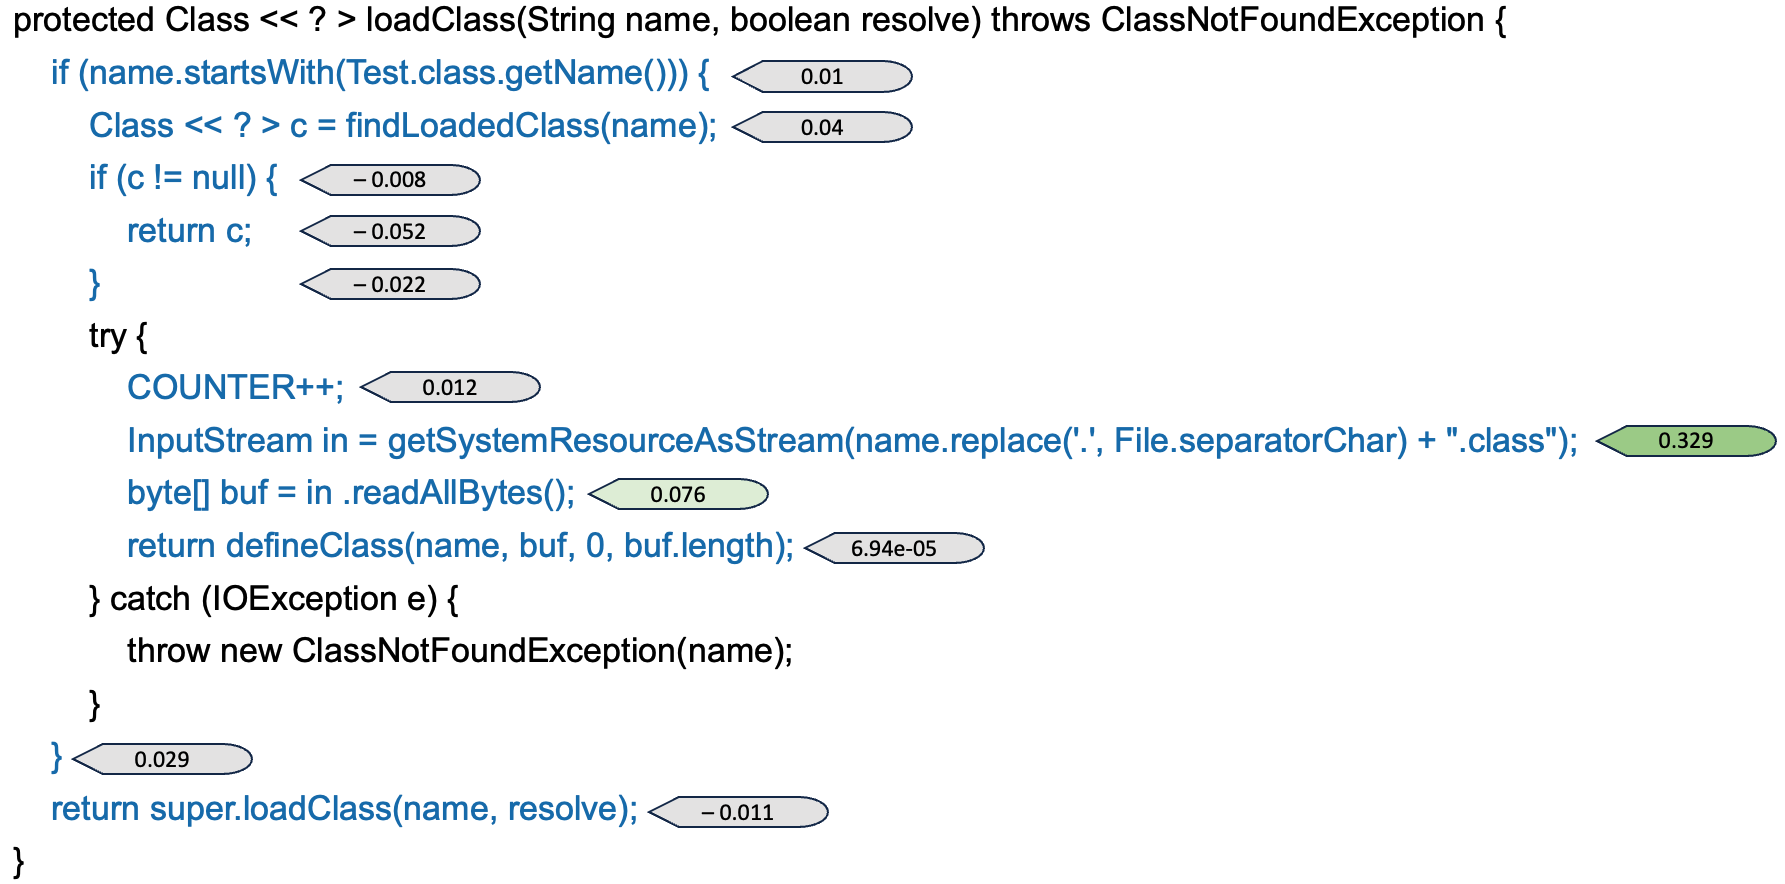
\includegraphics[width=3.4in]{rq1-case-study.png}
        \vspace{-20pt}
 	\caption{{\xblock} Case Study}
 	\label{fig:rq1-case}	
\end{figure}

\noindent {\bf Attribution Scores.} To illustrate how {\xblock} makes
the prediction, in Figure~\ref{fig:rq1-case}, we shows a code snippet
that catches an \code{IOException} thrown by the \code{readAllBytes}
API call on an \code{InputStream} object. CodeBERT produces as a
by-product an {\em attribution score} for each code sub-token in the
input. The higher the score of a token the higher attention that the
model pays to that token, contributing to the prediction result. In
Figure~\ref{fig:rq1-case}, for each statement, we show the statement
attribution score, which is calculated by averaging the attribution
scores of all the sub-tokens in the statement.
%The number after each statement is the statement attribution score,
%which is calculated by averaging the attribution scores of all the
%sub-tokens in the statement.
%
A positive attribution score means that the statement contributes
positively to the model's predicted class, while a negative score
means the statement contributes negatively to the predicted class.
As seen, the two statements that receive the highest scores are the
statement that defines the \code{InputStream} variable and the
statement that invokes the \code{readAllBytes} method call on the
\code{InputStream} object. This example illustrates that the model
is able to put the attention on the right (sub)token
of the input to decide the need of the \code{try-catch} block.


\begin{table}[t]%[htpb]
  \caption{Try-Catch Necessity Checking Evaluated on Test Partitions by the Number Of Try-Catch Blocks (RQ1) }
  \vspace{-12pt}
  \small
	\begin{center}
		\renewcommand{\arraystretch}{1}
		\begin{tabular}{| p{1.0cm}<{\centering} | p{0.7cm}<{\centering} | p{0.7cm}<{\centering}| p{0.7cm}<{\centering} | p{0.7cm}<{\centering} | p{0.7cm}<{\centering} | p{0.7cm}<{\centering} | }
		  \hline
			\multirow{2}{*}{} & \multicolumn{6}{c|}{Number of Try-Catch Blocks (Github dataset)} \\
			\cline{2-7}
			  & Zero  & One & Two & Three & Four & Five\\
			\hline
			Precision & 0.0 &  1.0 & 1.0 & 1.0 & 1.0 & 1.0\\
			\hline
			Recall   & 0.0 &  0.983 & 0.998 & 1.0 & 0.986 & 1.0\\
			\hline
			F1-score   & 0.0  &  0.991 & 0.999 & 1.0 & 0.993 & 1.0\\
			\hline
		\end{tabular}
		\label{tab:rq1-detailed-result}
	\end{center}
\end{table}

In addition, we partitioned the test dataset according to the number
of \code{try-catch} blocks, and evaluated {\xblock} on each
partition. As seen in Table~\ref{tab:rq1-detailed-result}, {\xblock}
gives 100\% correct prediction on the partitions with zero, three and
five \code{try-catch} blocks. Moreover, it achieves 100\% precision
and above 0.99 F1-score across all the partitions, showing that
{\xblock}'s prediction ability remains strong regardless of the number
of \code{try-catch} blocks in a code snippet.

%With a Precision of 68\%, it can decide correctly
%2 out of 3 cases if a code snippet needs a \code{try-catch}
%block or not. With a Recall of 79\%, {\tool} covers 4 out of
%5 cases that needs to be placed in a \code{try-catch} block. Users
%just need to find 1 out of 5 cases. As a result, it achieves a high
%F-score of 0.73.
%In FuzzyCatch dataset, {\tool} also achieves a high level of
%performance with XX\% precision, YY\% recall, and ZZ\% F-score.

%the state-of-the-art approach, XRank, {\bf -7.1\%} in Recall, {\bf
%  28.3\%} in Precision, and {\bf 12.3\%} in F-score.

%In FuzzyCatch dataset, the relative improvements are XX\%, YY\%, and
%ZZ\% in precision, recall, and F-score, respectively.

%We examined closely the cases that {\tool} performed better than
%XRank.

%Examining the result, we reported the following. First, if the
%association score of {\em only one API method} in the snippet and {\em one
%exception} is higher than a threshold, XRank decides that a
%\code{try-catch} block is needed.  Thus, it often tends to output
%  ``Yes''. {\em Its recall is slightly
%  better, but precision is just marginally better than a coin toss
%  (0.53) in our balanced dataset. That leads to lower F-score than {\tool}}.
%%
%Second,
%%XRank relies on the association scores between the presence of
%%API method calls and the presence of a \code{try-catch} block.
%the decisions on the necessity of a \code{try-catch} block or the
%exception types depend on the pre-defined thresholds in XRank on those
%association scores. Thus, those pre-defined thresholds might not be
%suitable across the libraries. Third, for the incomplete code
%snippets in which the names of the API methods in different packages
%or libraries are the same (e.g., \code{toString} or \code{getText} in
%various JDK packages), XRank cannot distinguish them and use one entry
%in the dictionary for them due to its IR approach. In contrast, unlike
%XRank which considers only the API method calls in a \code{try-catch}
%block, {\tool} considers the code in the block as the context to learn
%the program dependencies/relations among the names of those API
%elements. That is, it leverages the relations among the names of API
%elements to learn their identities, thus, deciding better the need of
%\code{try-catch} blocks and the corresponding exception types.

%Tien:RQ2 Table
%\begin{table}[t]
%  \caption{Try-Catch Statement Detection Effectiveness (RQ2)}
%  \vspace{-12pt}
%	\begin{center}
%		\small
%		\renewcommand{\arraystretch}{1} 
%		\begin{tabular}{p{0.8cm}<{\centering}|p{0.4cm}<{\centering}|p{0.4cm}<{\centering}|p{0.4cm}<{\centering}|p{0.4cm}<{\centering}|p{0.4cm}<{\centering}|p{0.4cm}<{\centering}|p{0.4cm}<{\centering}|p{0.4cm}<{\centering}|p{0.4cm}<{\centering}|p{0.4cm}<{\centering}}
%			\hline
%			 	&  \multicolumn{10}{c}{Accuracy} \\
%			\cline{2-11}
%			     	&  N1  & N2   &  N3  & N4   &N5    & N6   &N7    & N8   &N9    & N10 \\
%			\hline
%			\tool     & 0.42 & 0.47 & 0.59 & 0.66 & 0.71 & 0.74 & 0.76 & 0.77 & 0.78  & 0.79  \\
%			\hline
%		\end{tabular}
%		Nx is number of nodes in the explanation
%                sub-graph (\code{try-catch} block)
%		\label{tab:rq2}
%	\end{center}
%\end{table}


%Take as an example a code snippet (not shown) in our dataset with the
%presence of \code{getText}. This name is popular with a very large number
%of API method candidates.
%%For example, in a code snippet, \code{getText} has a very large number
%%of API method candidates.
%However, considering the relation between \code{css} and
%\code{getText} in the code \code{`...css()\-.getText()'},~the number
%of candidates for \code{getText} is only 4. Finally, considering~the
%return value of \code{getText} as an argument of
%\code{setInnerText(...)} in the code
%\code{`setInnerText(...css()\-.getText())'}, only one candidate is
%remained:
%\code{com\-.google\-.gwt\-.resources\-.client\-.CssResource\-.getText()}.
%Thus, those relations actually help identify the API elements,
%leading to better decision in {\tool} on the \code{try-catch} block
%and exception types.
%%
%Because it has not seen any \code{try-catch} block involving
%\code{com\-.....getText()} and those related ones, {\tool} decides
%that the code snippet does not need a \code{try-catch} block. In
%contrast, XRank considers only the {\em pairwise} associate scores
%between an {\em individual API method call} and the exception types
%in a \code{catch} clause. It disregards those above
%relations/dependencies among the API names. Thus, it might
%misunderstand that \code{getText} needs a \code{try-catch} due to the
%co-occurrences of other API elements that need one. That is, without
%the dependencies, XRank might make incorrect identification of the API
%elements via their names, leading to incorrect exception
%recommendation.

%considering Groum but only to get better API ...


%\begin{table}[htpb]
%  \caption{Try-Catch Necessity Checking Comparison (RQ1)}
%  \vspace{-12pt}
%	\begin{center}
%		\renewcommand{\arraystretch}{1}
%		\begin{tabular}{p{1.5cm}<{\centering}|p{1.25cm}<{\centering}p{1.25cm}<{\centering}|p{1.25cm}<{\centering}p{1.25cm}<{\centering}}
%			\hline
%			\multirow{2}{*}{} & \multicolumn{2}{c|}{{\tool} Dataset} & \multicolumn{2}{c}{FuzzyCatch Dataset}\\
%			\cline{2-5}
%			  & \tool  & XRank & \tool  & XRank\\
%			\hline
%			Recall    & \textbf{0.81} & &&\\
%			Precision & \textbf{0.66} & &&\\
%			F-score   & \textbf{0.73} & &&\\
%			\hline
%		\end{tabular}
%		\label{tab:xblock}
%	\end{center}
%\end{table}
